\documentclass[../../../Bachelorarbeit.tex]{subfiles}
\begin{document}

\subsection{Stromlaufplan} \label{Stromlaufplan}
% \color{red}
% Ausschnitte des Stromlaufplanes mit besonderer Relevanz einfügen und erklären !!!
Dieses Unterkapitel soll einen Überblick zur Entwicklung des Stromlaufplanes geben. Ziel des Überblickes ist nicht den kompletten Stromlaufplan darzustellen und zu erklären, sondern auf besonders relevante Aspekte in der Verdrahtung Bezug zu nehmen. Der vollständige Stromlaufplan des Systems kann im Anhang (siehe \autoref{anhang}Anhang) wiedergefunden werden. Auf die Verdrahtung der Feld- und Prozessebene wird in diesem Abschnitt nicht eingegangen.\\
Zunächst wird der Anschluss des Netzteils \acs{lxm}62P dargestellt. Grundlegend braucht das Netzteil eine 400 \si{V} Wechselstromversorgung und eine 24 \si{V} Gleichstromversorgung. Erstere stellt die Spannungsversorgung für die an den Servoregler angeschlossenen Motoren dar. Der 24 \si{V} Anschluss wird für die Steuerungsebene benötigt. \autoref{fig:my-img100} zeigt die geforderte Verdrahtung des Netzteils. 

\begin{figure}[H]
    \centering
    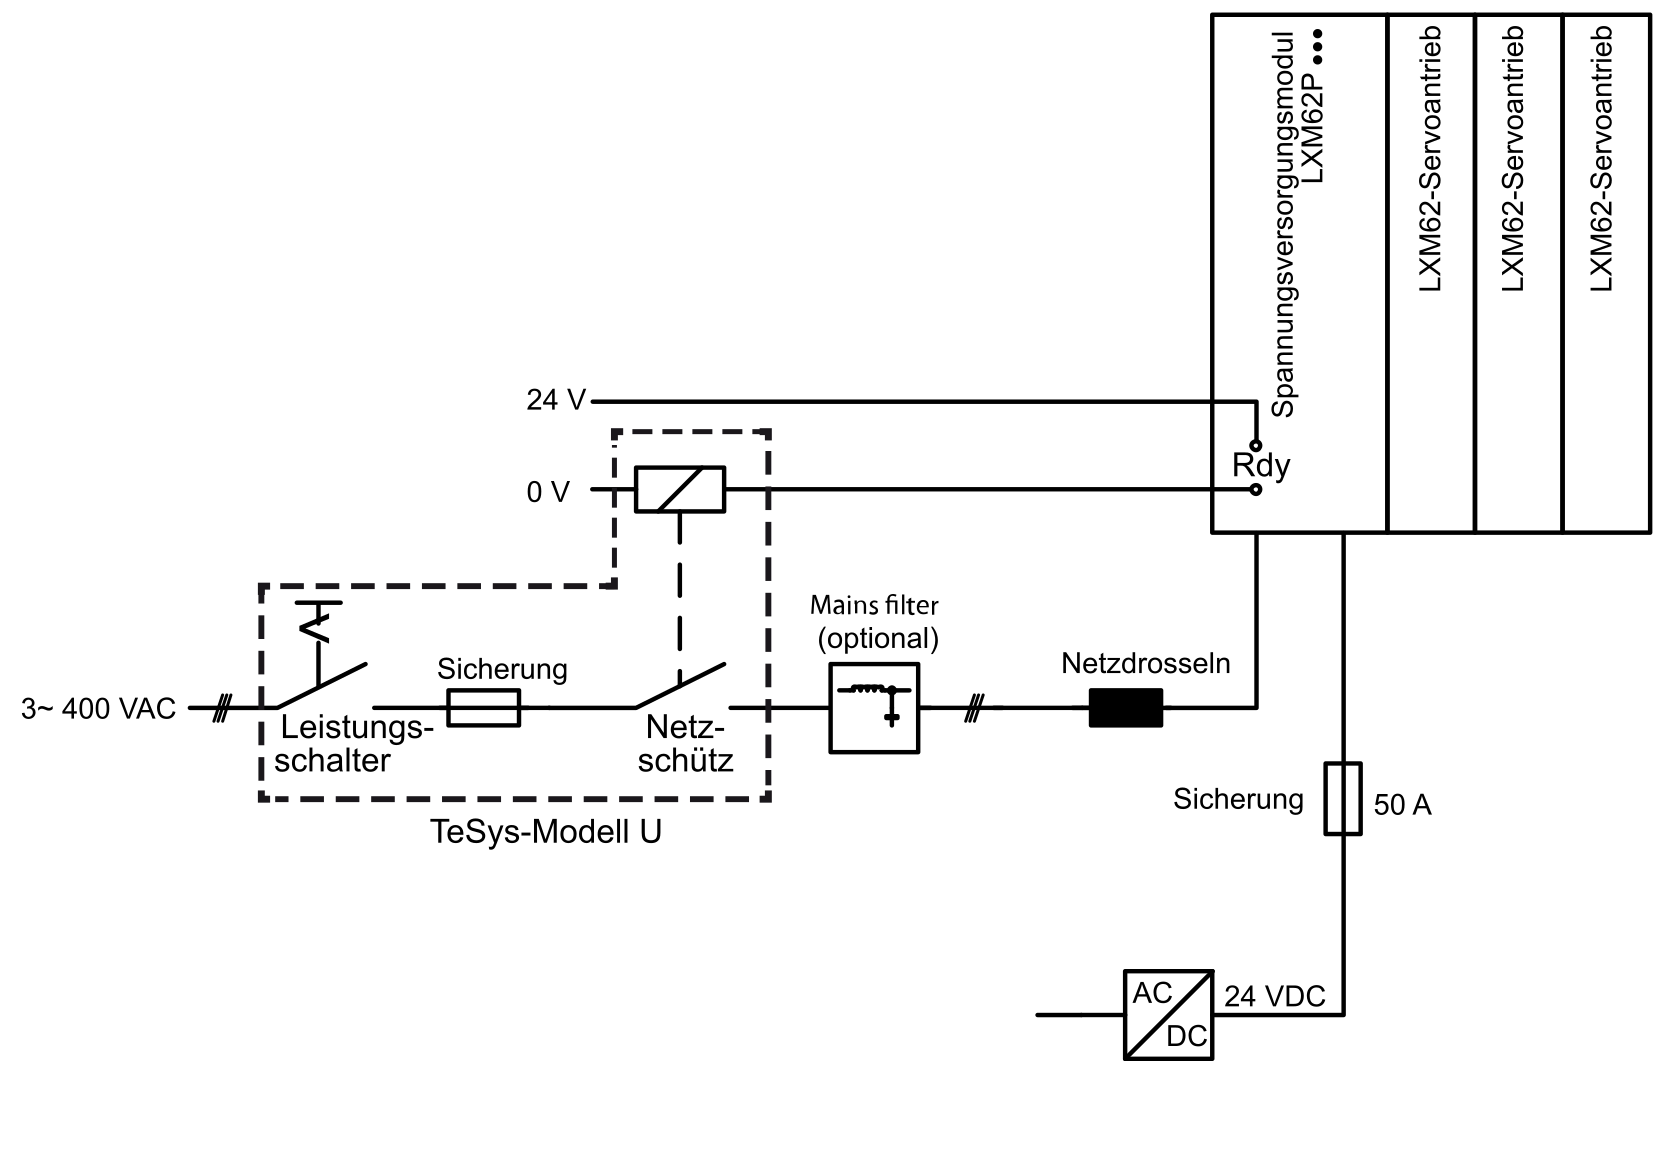
\includegraphics[width=0.9\textwidth]{Images/netzteil_verdrahtung.png}
    \caption[Netzteilverdrahtung]{Anschluss und Verdrahtung des Netzteils LXM62P}
    \label{fig:my-img100}
\end{figure}

Zu erkennen ist ein Netzschütz, welches die 400 \si{V} Ebene im Ready-Zustand des Systems über ein Schütz schalten kann. Grund für diese Implementation ist die Forderung des Zuschaltens der Versorgungsspannung erst bei Bedarf (wenn positioniert werden soll). Ziel ist die Verbesserung der Sicherheit des Systems. Der Mains-Filter und die Netzdrossel dienen zum Kompensieren von Oberschwingungen und der Glättung des Netzes.\\
\smallskip \newline
Auch der Anschluss des Servoreglers \acs{lxm}62D bedarf einer eigenen Betrachtung. Grund ist die Berücksichtigung der funktionalen Sicherheit des Servoreglers und der an diesem angeschlossenen Motoren. Grundlegend soll der Servoregler über den Inverter-Enable Eingang aktiviert \bzw deaktiviert werden. Der aktivierte Zustand muss dabei aktiv über die Bestromung des Eingangs hergestellt werden. Dies geschieht über einen sicheren Ausgang am \acs{slc}. Der Ausgang wird im Fehlerfall deaktiviert, was dafür sorgt, dass auch der Inverter-Enable Anschluss am Regler nicht mehr versorgt wird und letztendlich zur Abschaltung des Servoreglers führt. Die folgenden zwei Grafiken zeigen den Steuerkreis (siehe \autoref{fig:my-img101}) und den Lastkreis (siehe \autoref{fig:my-img102}) zur Implementation besagter Funktionalität.
\clearpage

\begin{figure}[H]
    \centering
    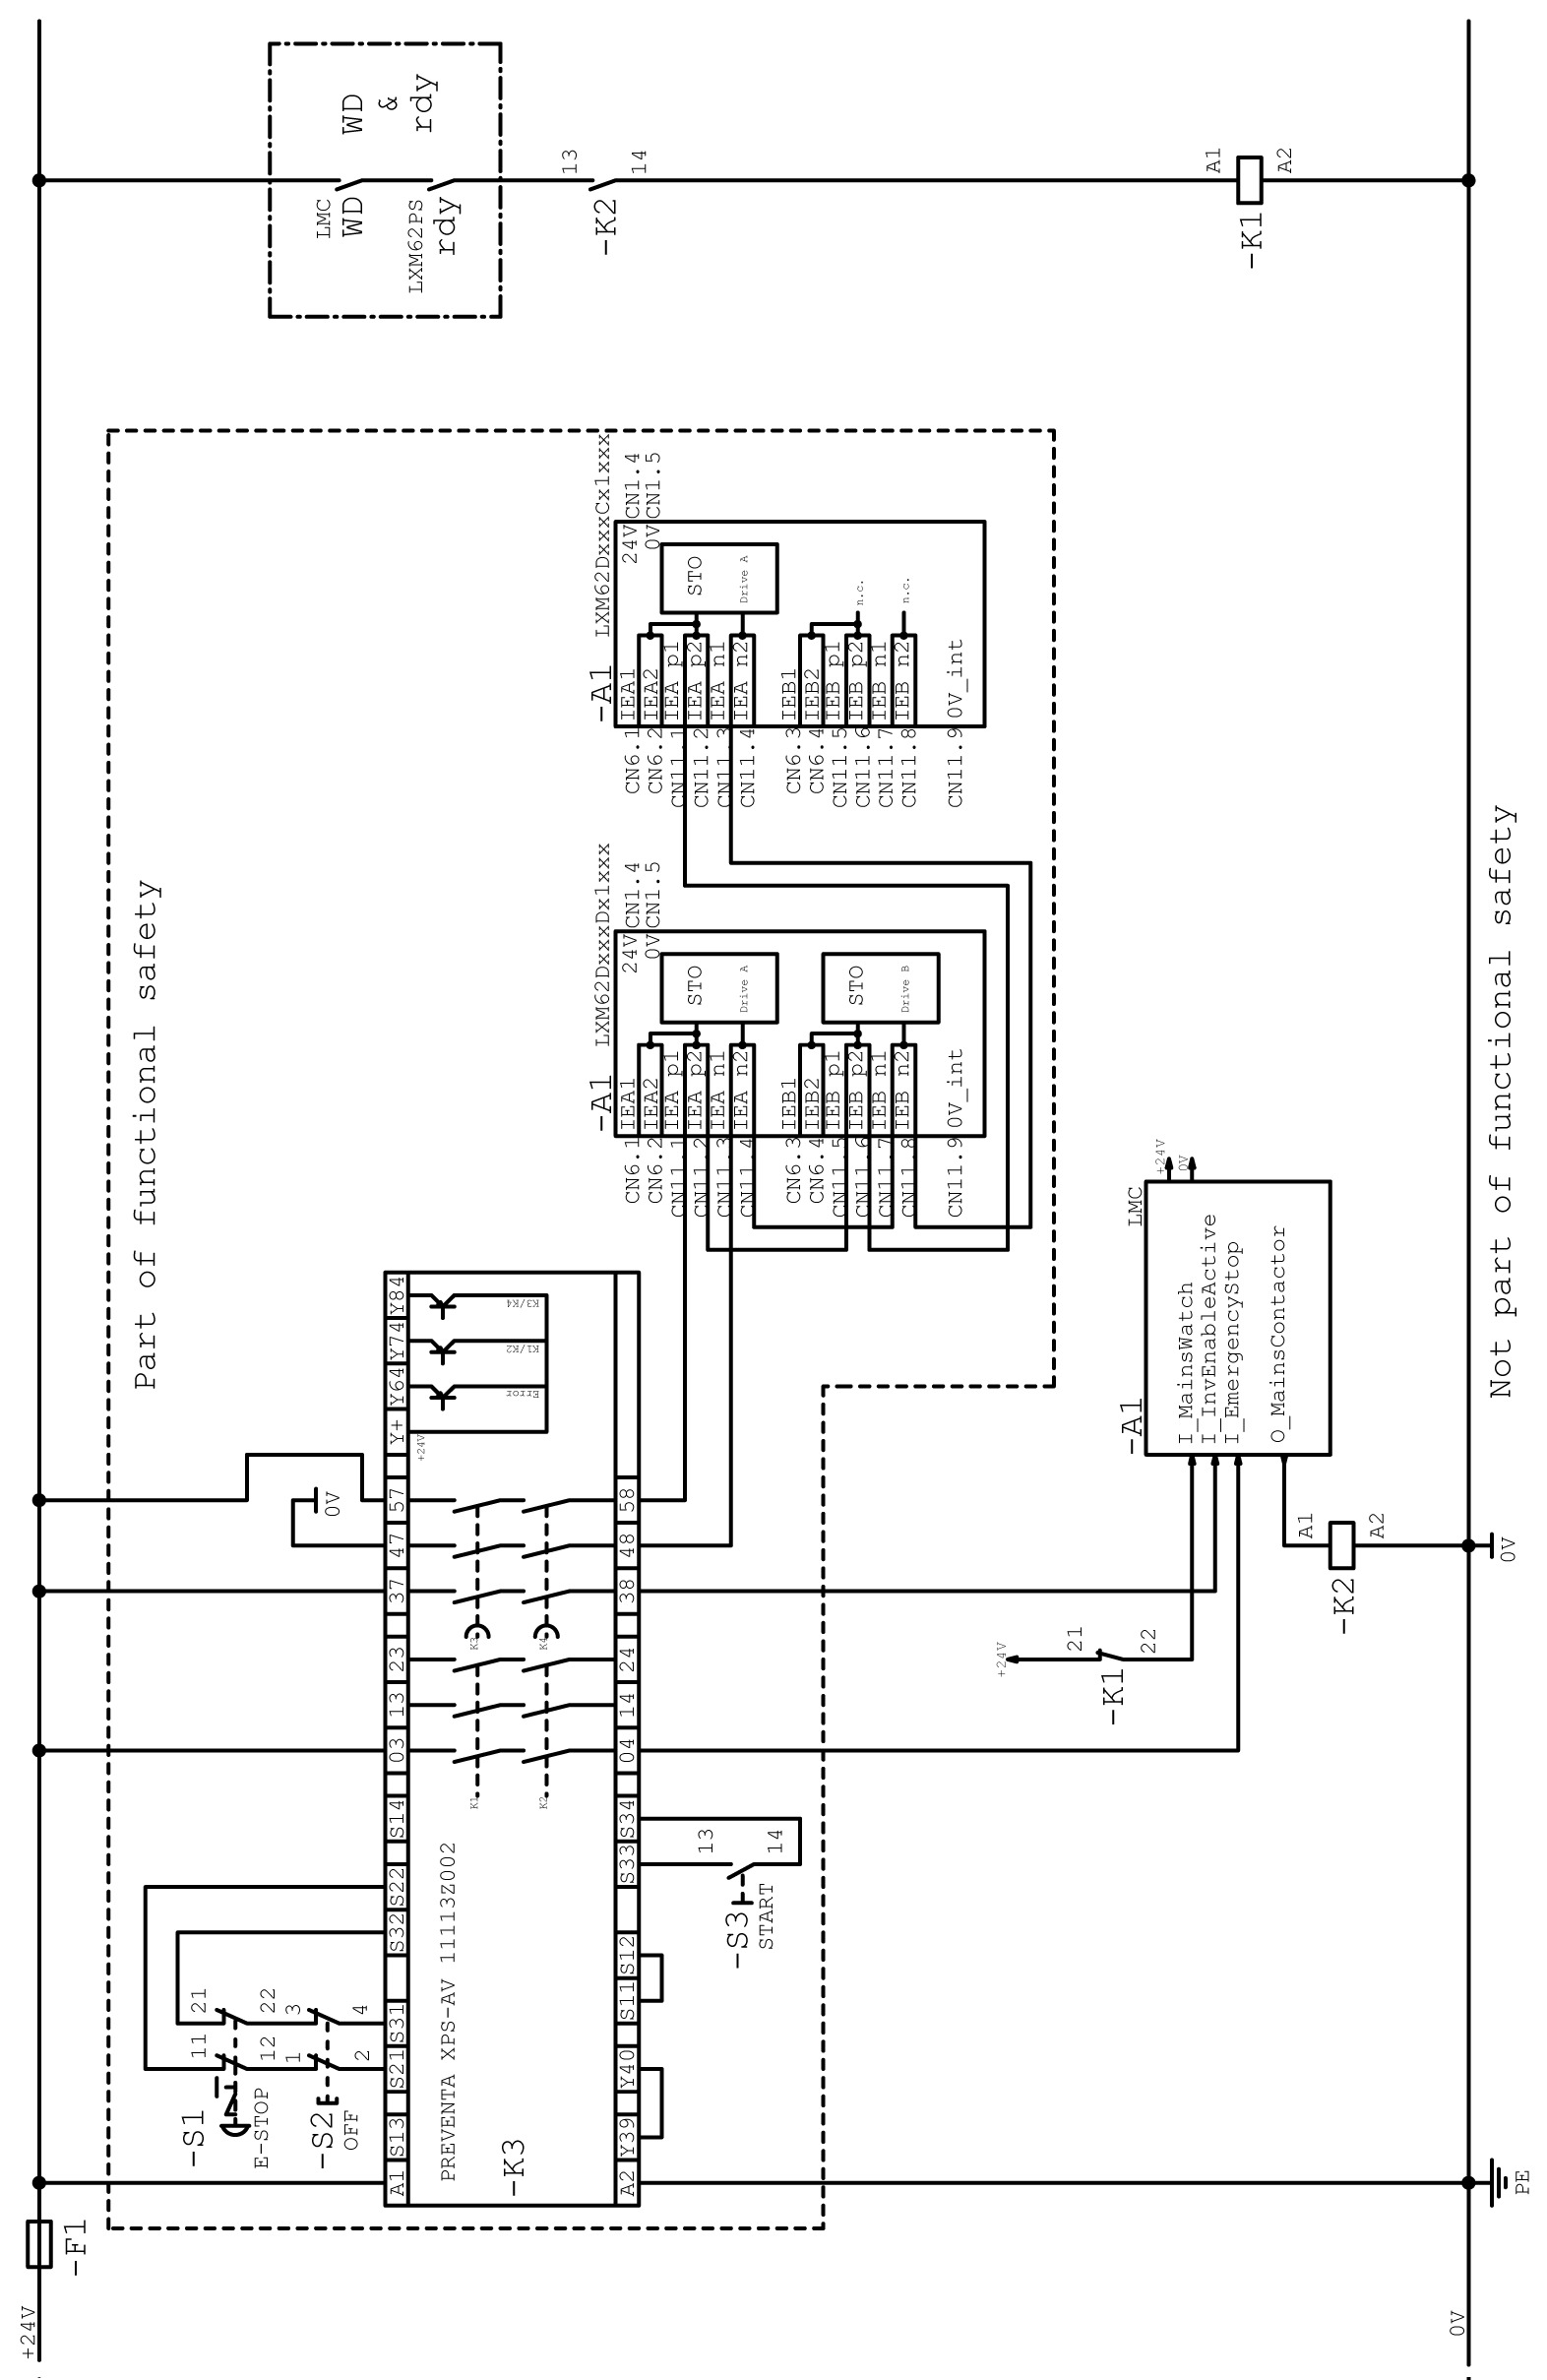
\includegraphics[width=0.8\textwidth]{Images/steuerkreis.jpg}
    \caption[Steuerkreis Servoregler]{Steuerkreis des Servoreglers LXM62D}
    \label{fig:my-img101}
\end{figure}

\begin{figure}[H]
    \centering
    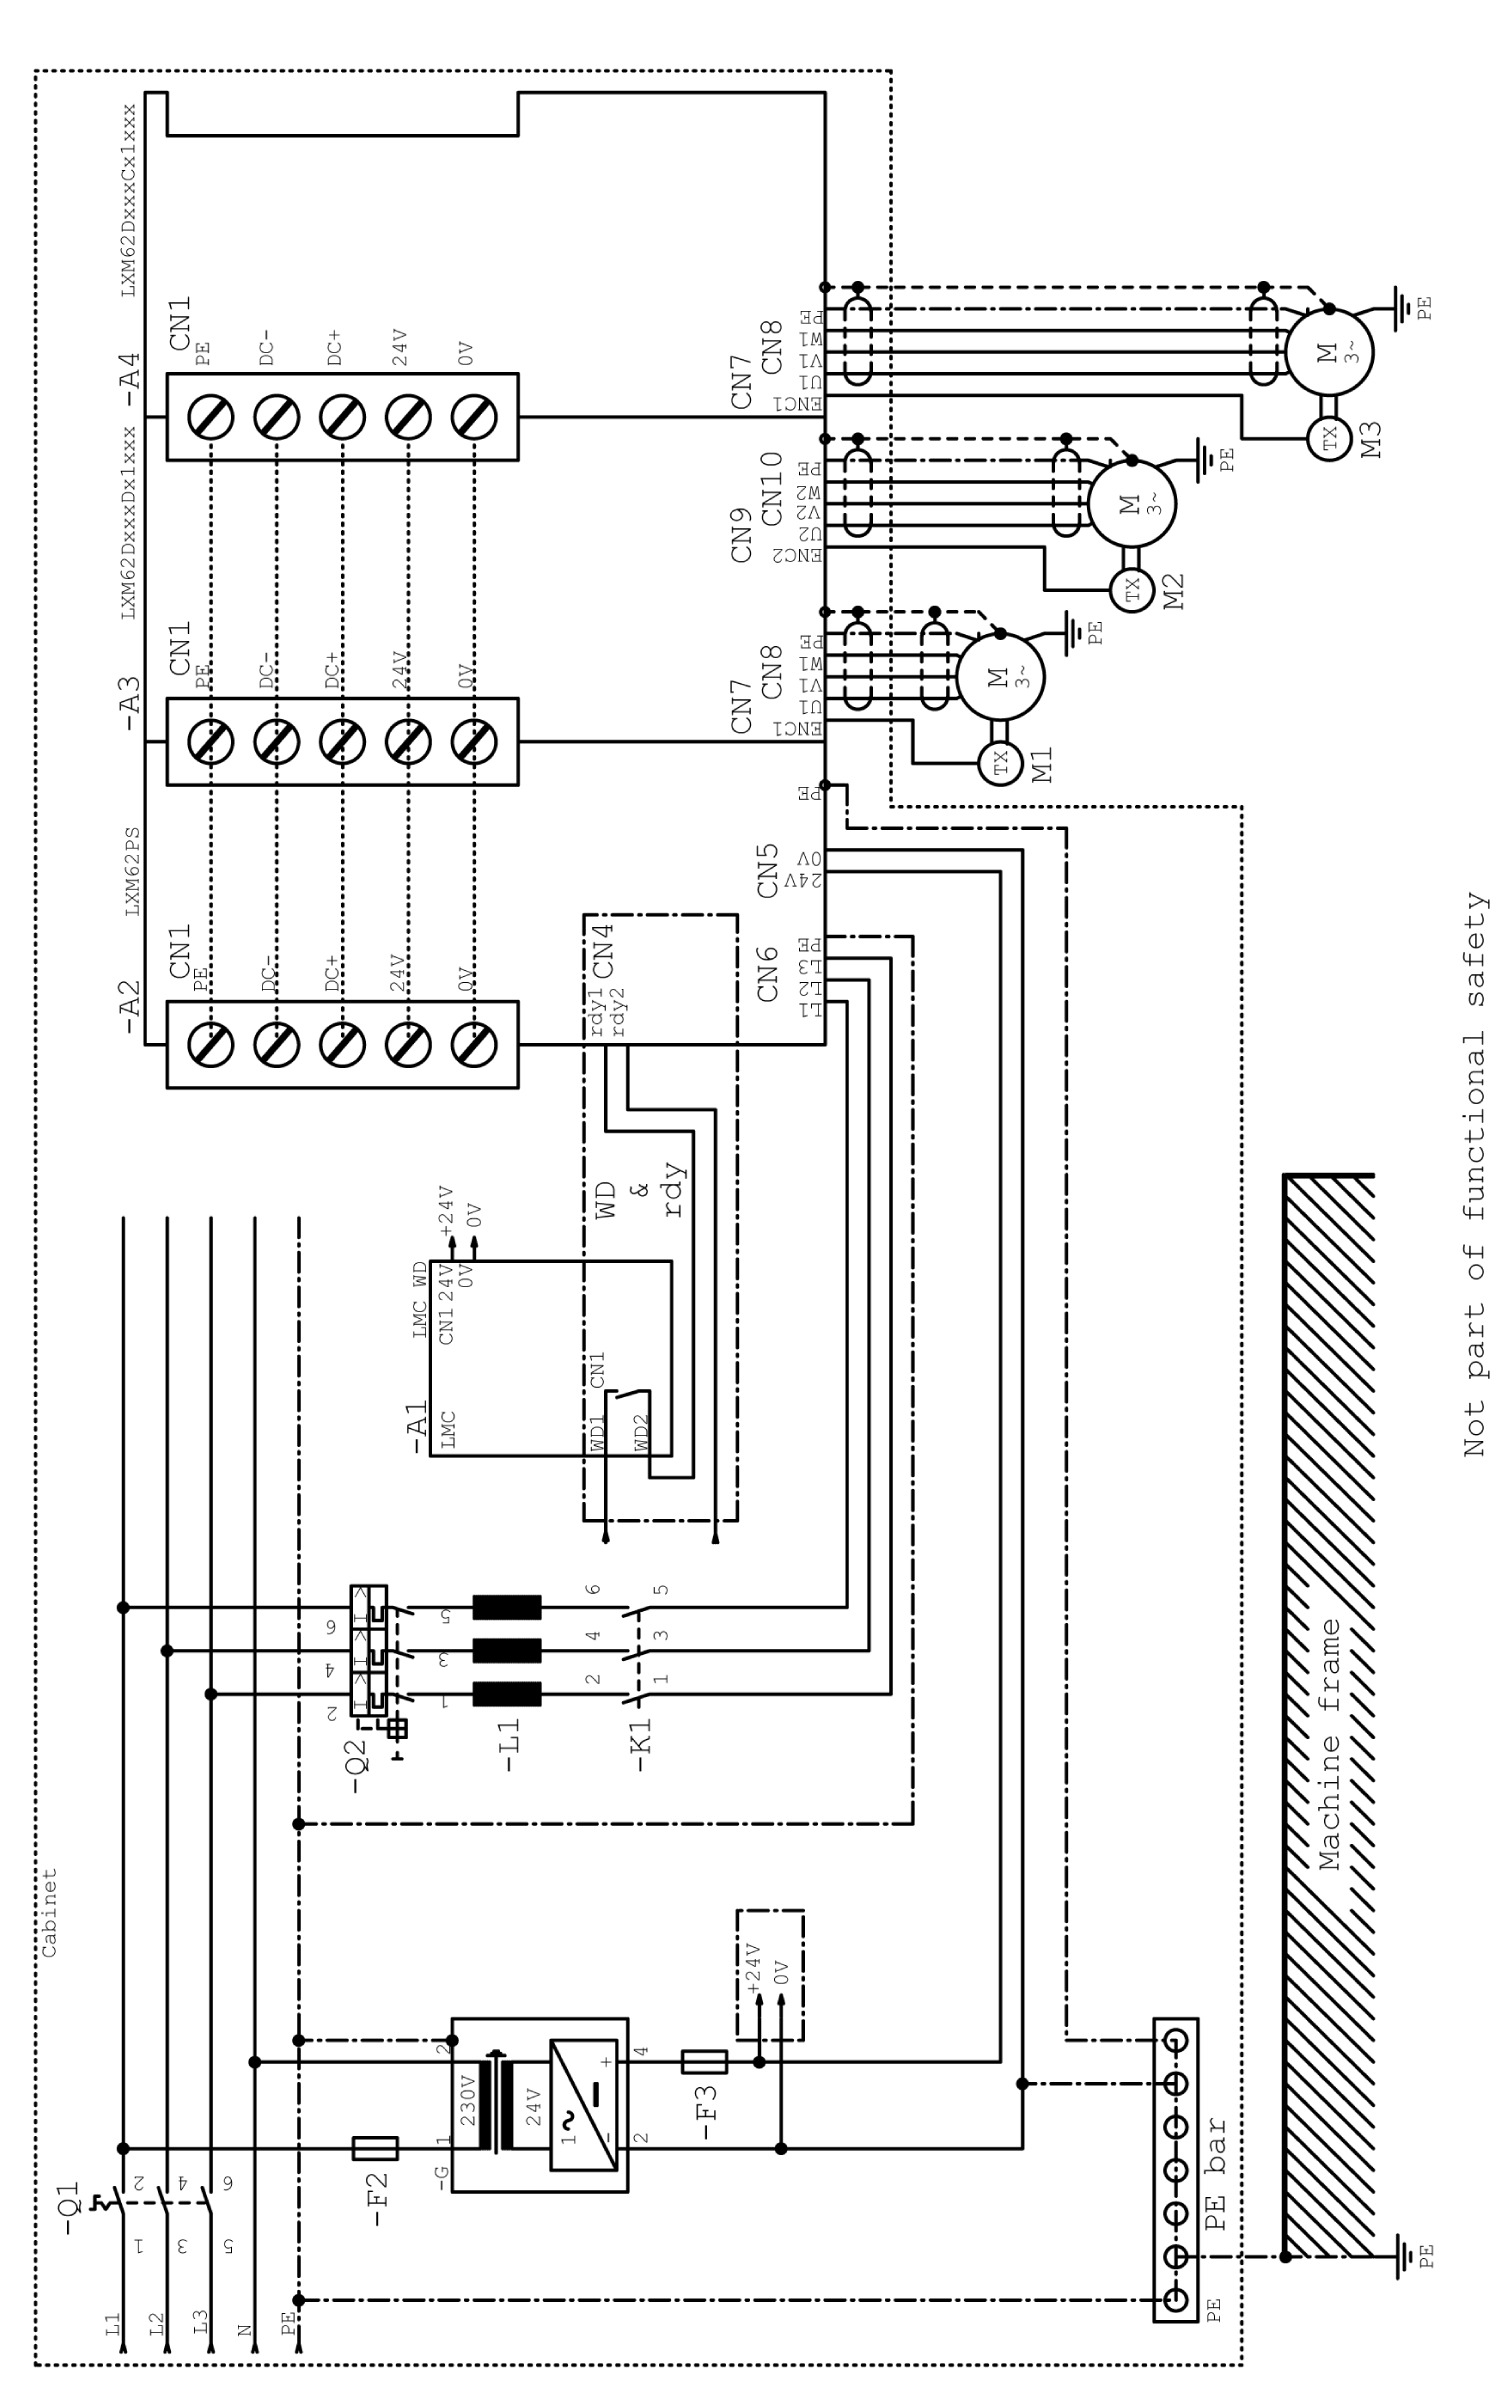
\includegraphics[width=0.8\textwidth]{Images/lastkreis.jpg}
    \caption[Lastkreis Servoregler]{Lastkreis des Servoreglers LXM62D}
    \label{fig:my-img102}
\end{figure}

\end{document}